\documentclass[aspectratio=169]{beamer}
\usepackage{../theme/cs2theme}
\usepackage{../theme/cs2commands}
\usepackage{graphicx}
\setcsweek{Week 3}
\title{Run It. Then Measure It.}
\subtitle{Open lab: local models, variance, and the Foreman/Worker pair}
\author{Computer Science II \textbullet\ Dr. Jeremy P. Evert}
\date{September 2, 2026}
\graphicspath{{img/}}
\begin{document}
\begin{frame}[plain]\titlepage\end{frame}
\begin{destinationframe}{Today's destination}
  \begin{itemize}
    \item Actually get a local model talking back to you, not just installed.
    \item Split Foreman/Worker roles and use them on purpose.
    \item Turn one World Bible scenario into a real prompt.
    \item Measure a model, not just watch it: variance and load time.
  \end{itemize}
\end{destinationframe}
\begin{frame}{Pick up where Monday left off}
  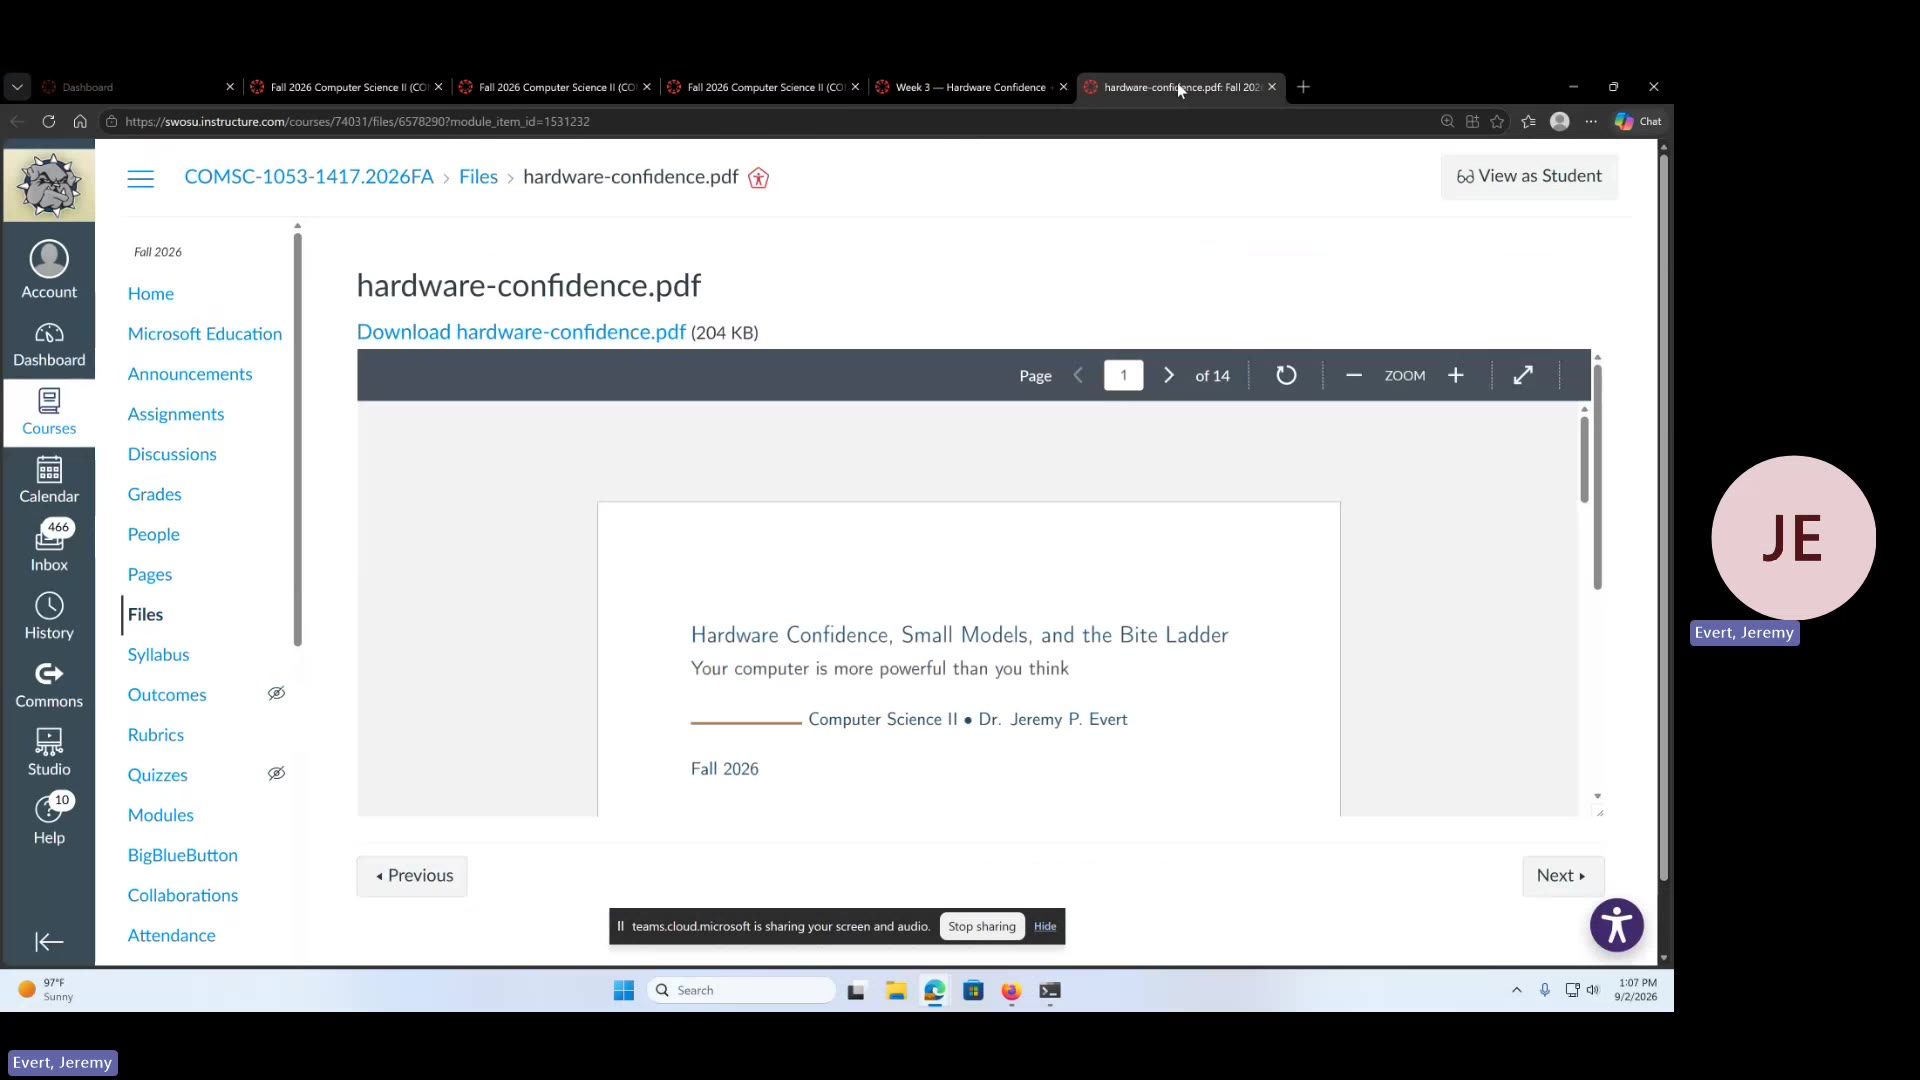
\includegraphics[width=.78\textwidth,height=.62\textheight,keepaspectratio]{monday_archive}
  \vfill\centering\small Monday's recording and slides stay linked in this module -- use them alongside today's lab.
\end{frame}
\begin{frame}{Foreman, Worker, Navigator}
  \begin{itemize}
    \item Worker drives the keyboard. Foreman narrates intent before acting.
    \item Foreman's real job: catch the moment the Worker notices something interesting and \emph{doesn't} stop to ask about it.
    \item That moment is exactly what gets pasted into Copilot or ChatGPT.
    \item Bonus points for the Foreman: get artifacts into GitHub, and keep lab notes.
  \end{itemize}
\end{frame}
\begin{frame}{Four worlds, four seeded inconsistencies}
  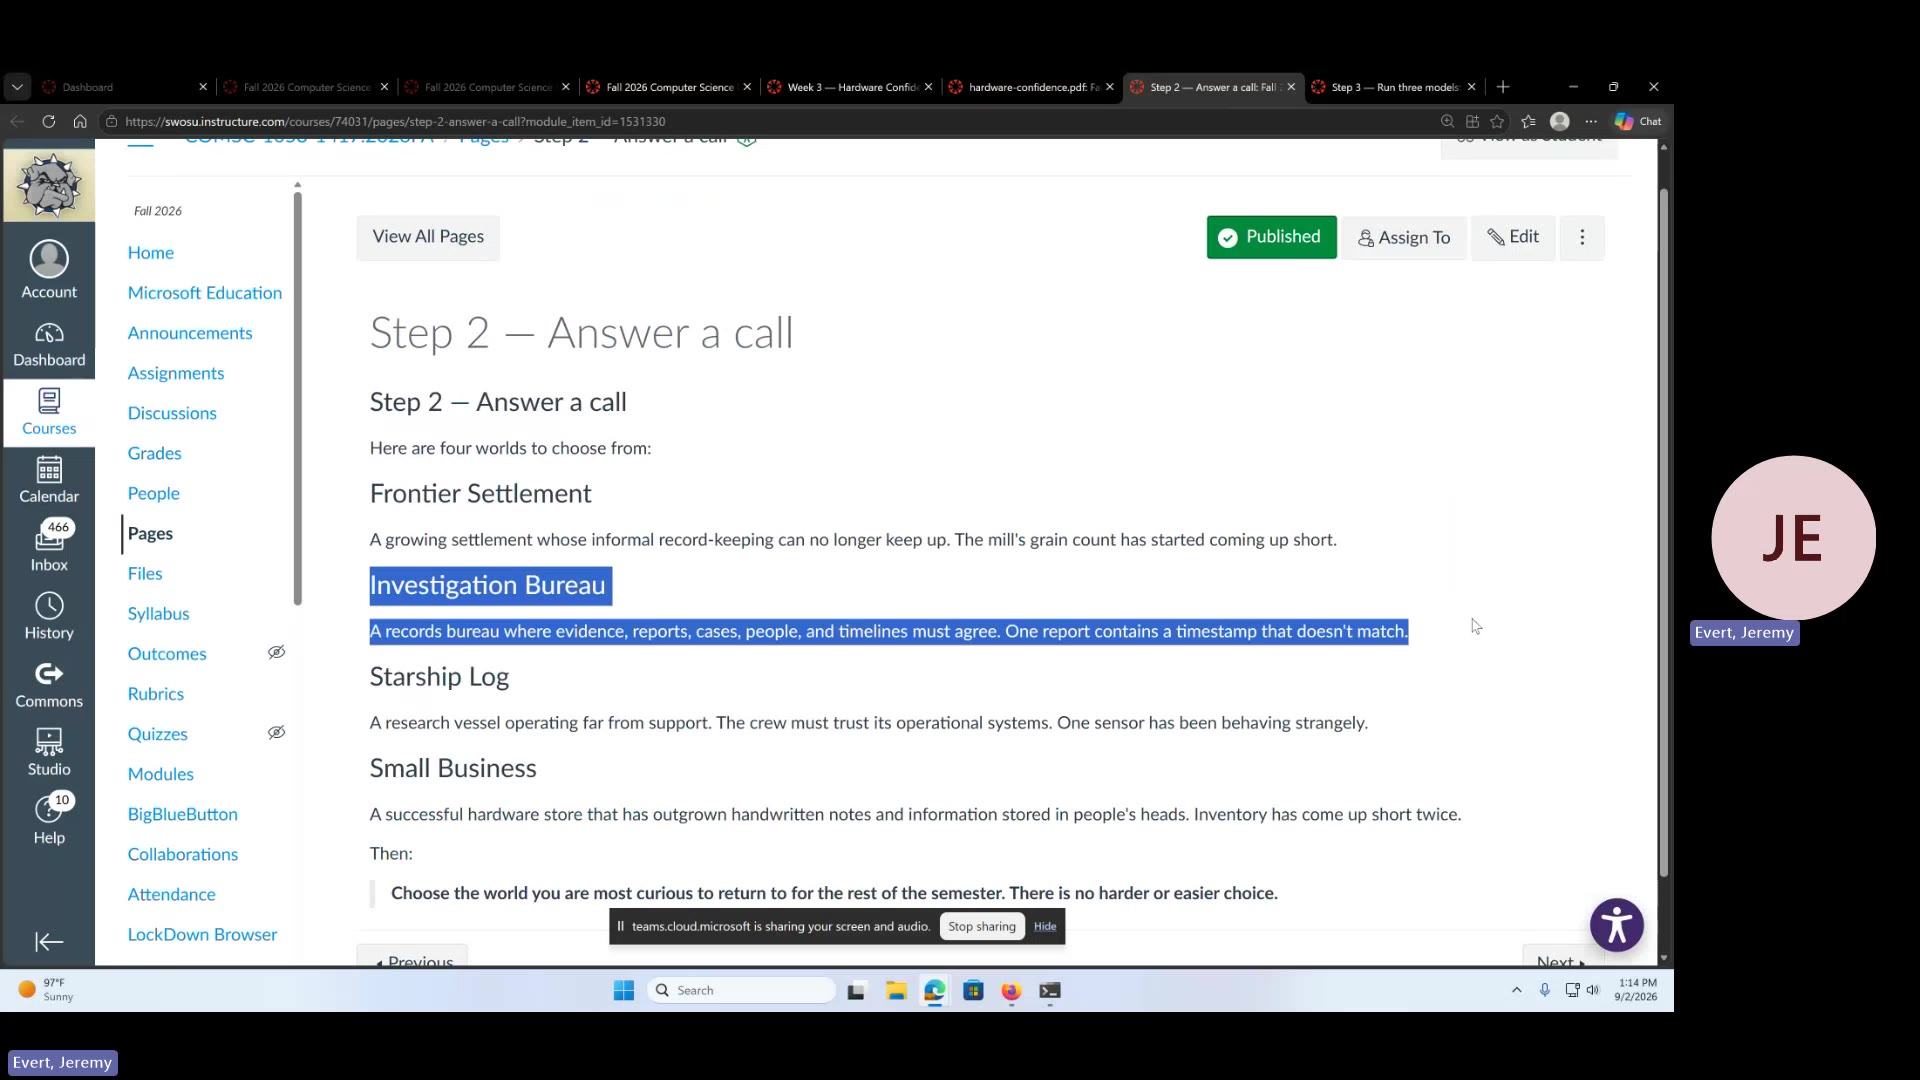
\includegraphics[width=.78\textwidth,height=.62\textheight,keepaspectratio]{answer_a_call}
  \vfill\centering\small Frontier Settlement, Investigation Bureau, Starship Log, Small Business -- each one ships with a mismatch to chase.
\end{frame}
\begin{frame}{Ask for a script -- then read it}
  \begin{columns}[T]
    \column{.48\textwidth}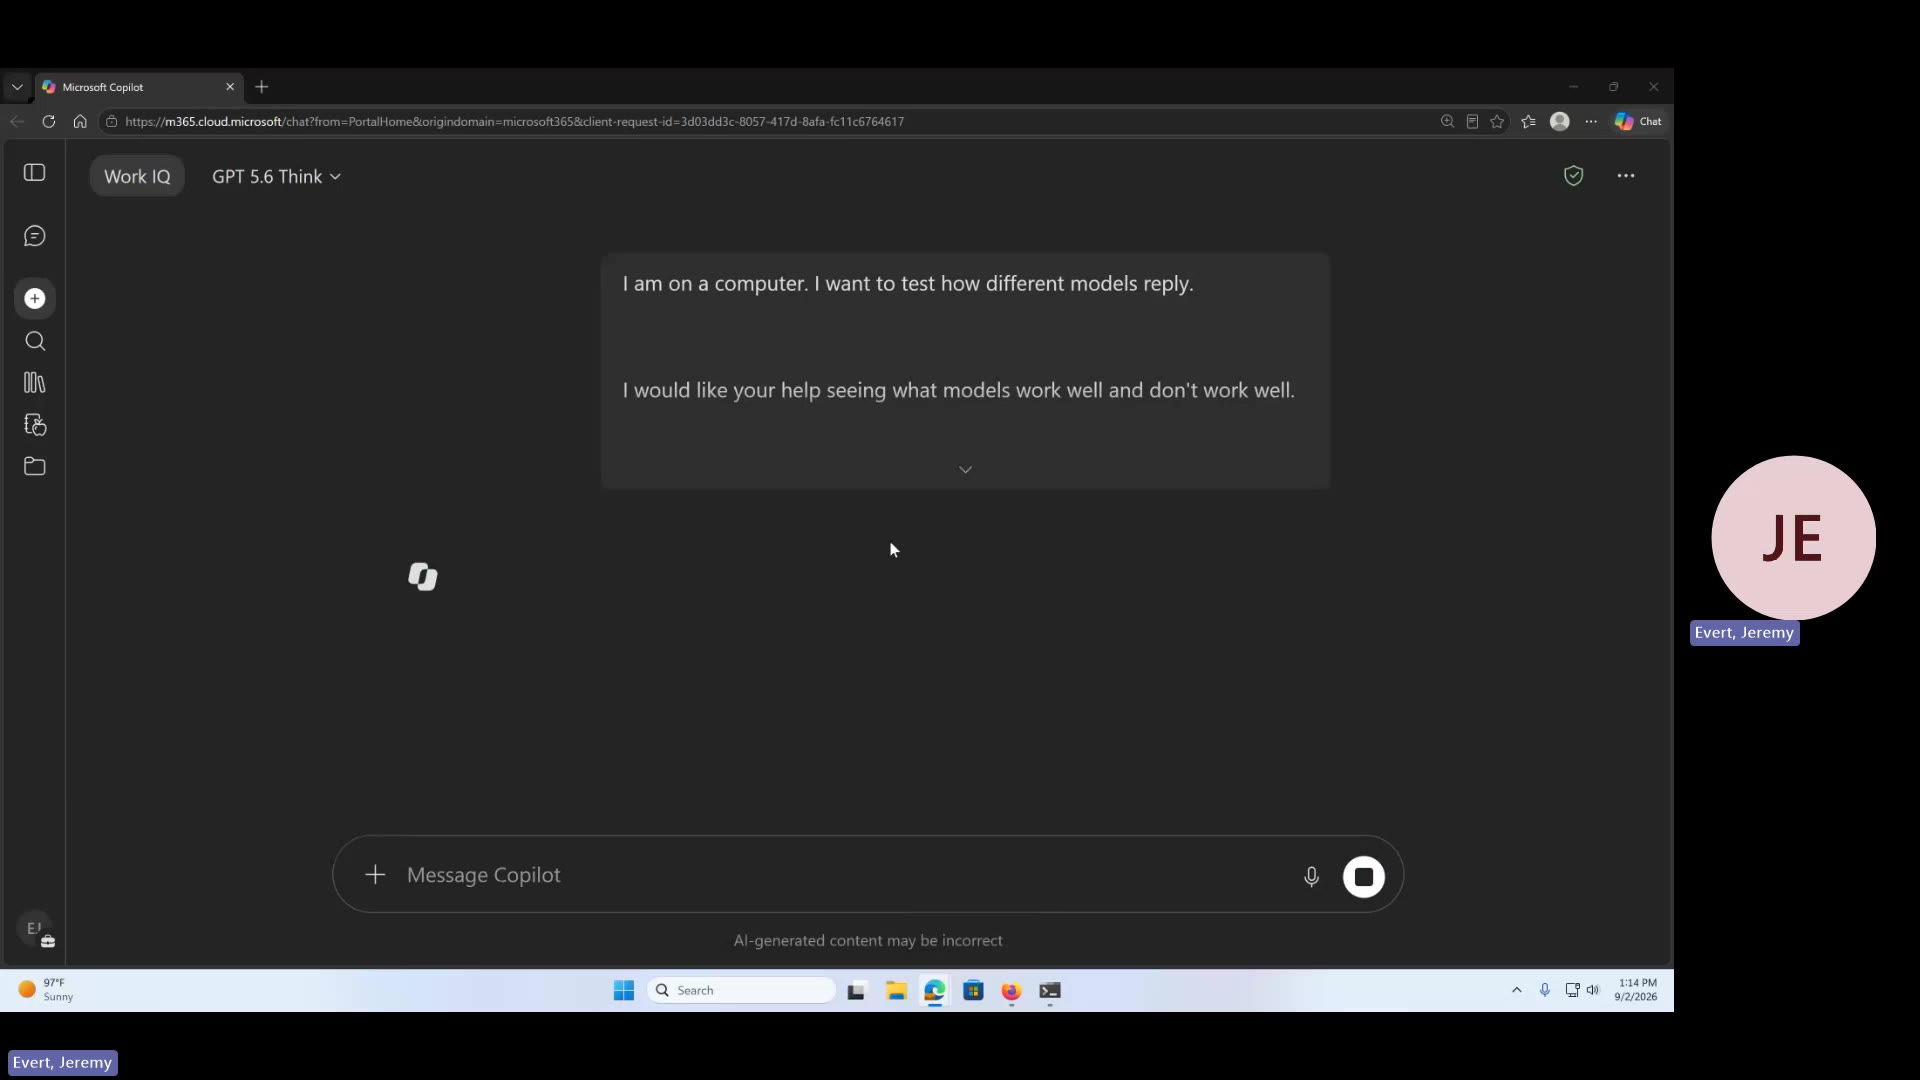
\includegraphics[width=\textwidth]{copilot_prompt}
    \column{.48\textwidth}\begin{itemize}\item Plain-language ask: “I am on a computer, I want to test how different models reply.”\item Copilot handed back a PowerShell scaffold.\item The habit that matters: read every line before you run it.\end{itemize}
  \end{columns}
\end{frame}
\begin{frame}{What the scaffold actually did}
  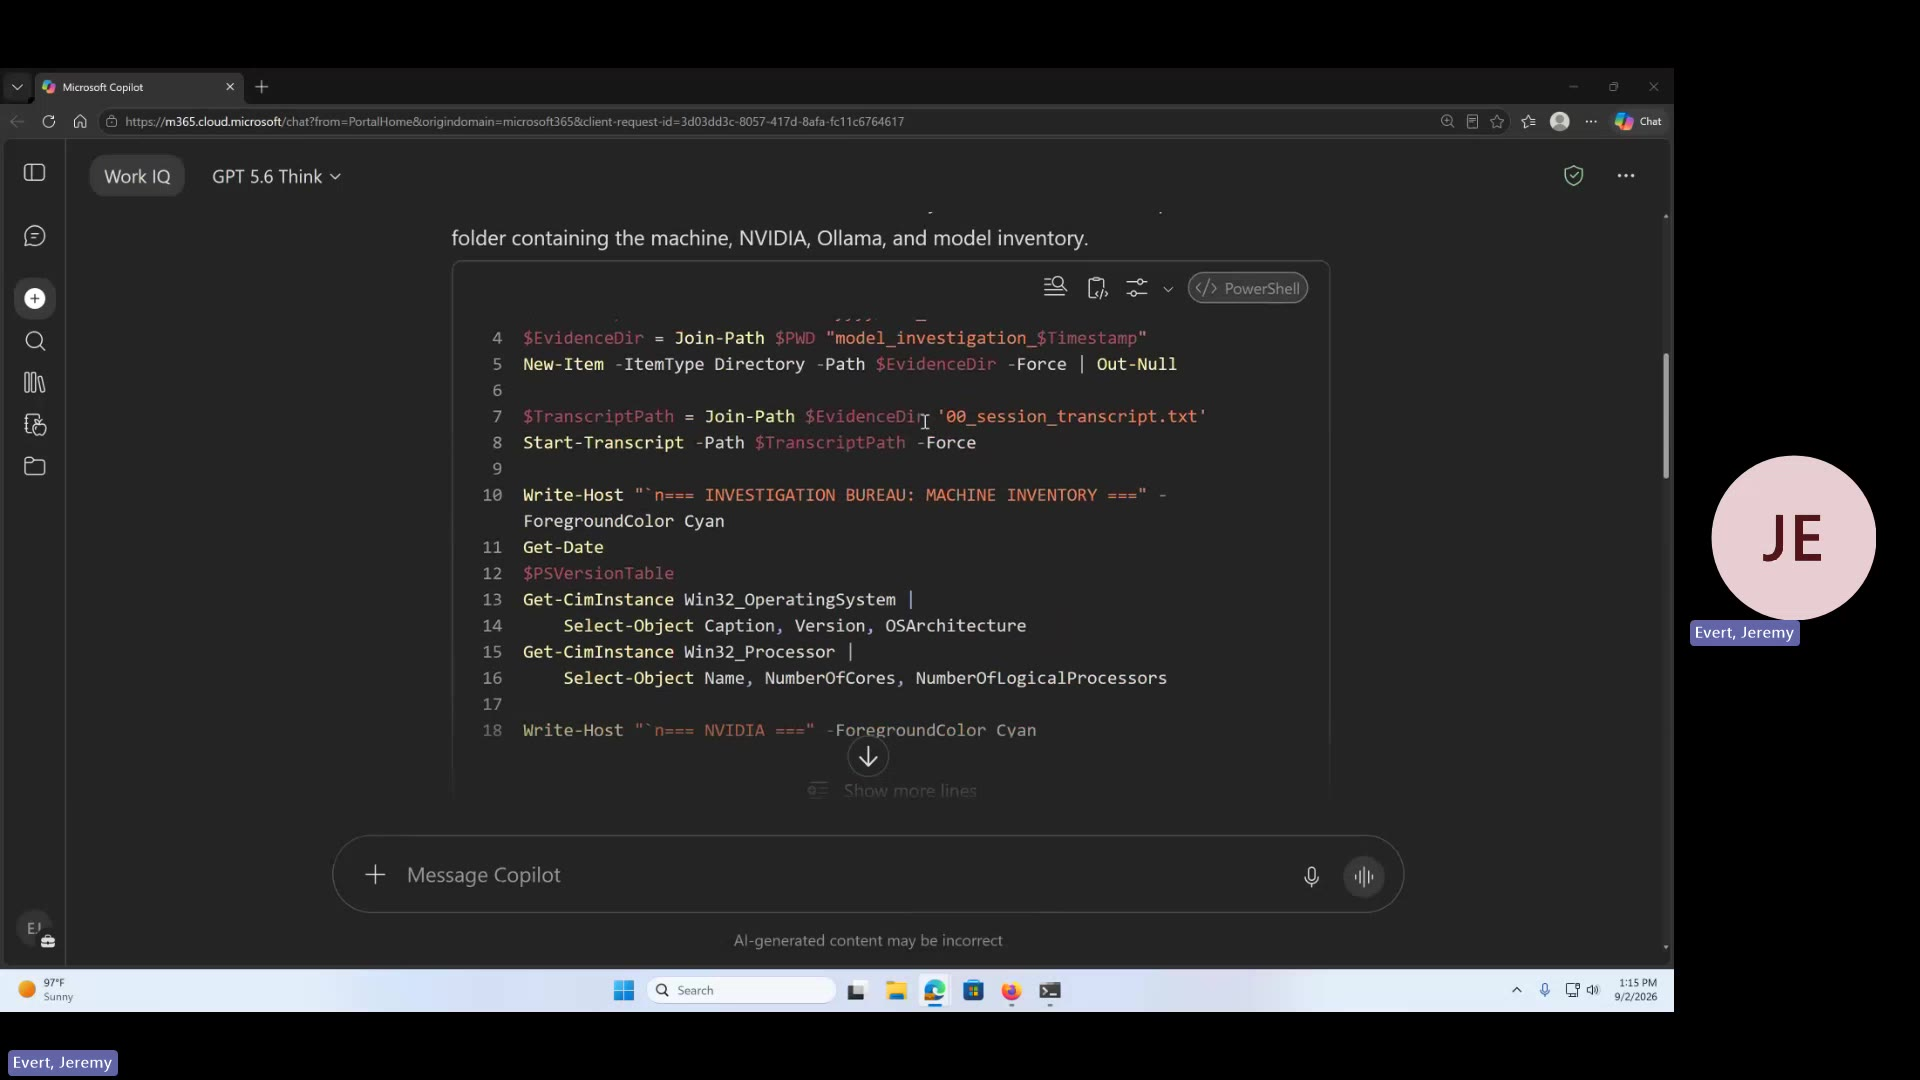
\includegraphics[width=.62\textwidth,height=.60\textheight,keepaspectratio]{copilot_script}
  \vfill\centering\small \texttt{Start-Transcript} to log the session, \texttt{Get-CimInstance} for machine info, an \texttt{nvidia-smi} block for GPU state.
\end{frame}
\begin{frame}{Read \texttt{nvidia-smi} before you blame the model}
  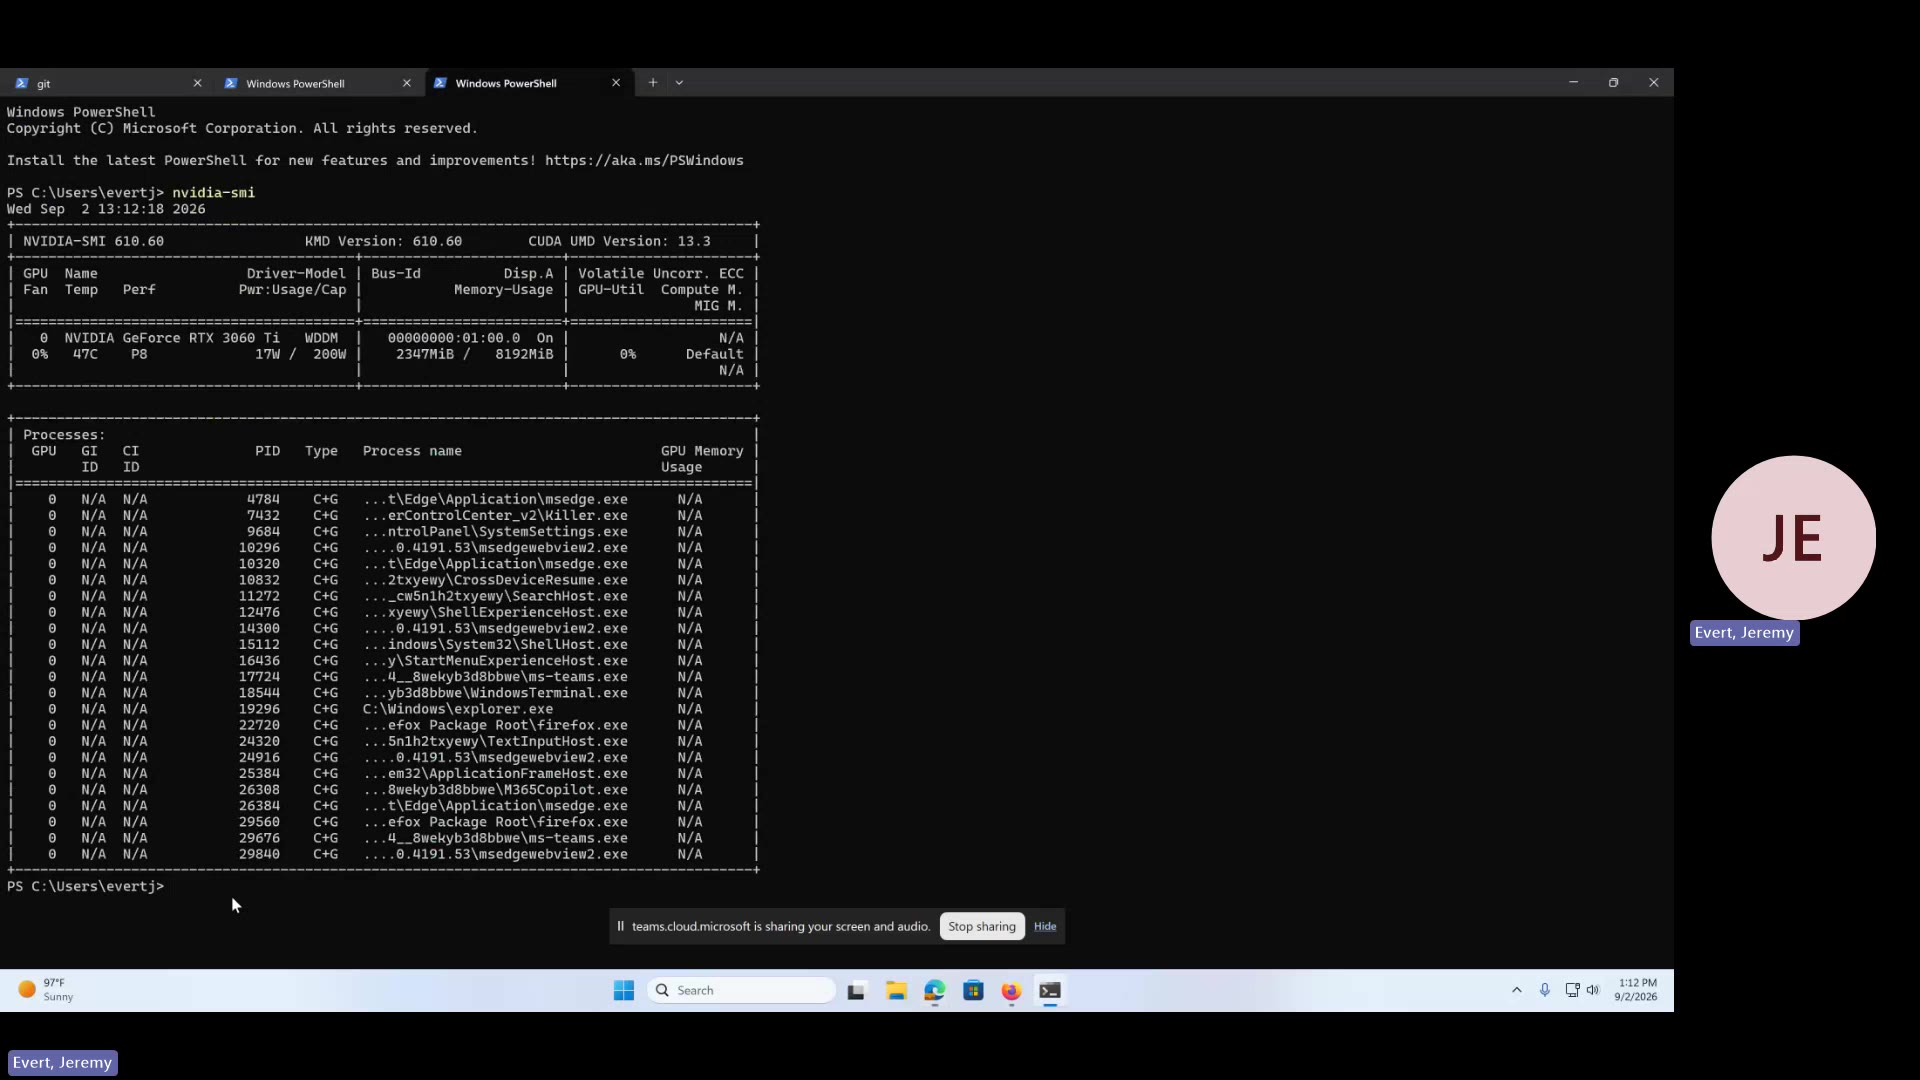
\includegraphics[width=.68\textwidth,height=.60\textheight,keepaspectratio]{gpu_status}
  \vfill\centering\small VRAM already in use at idle is real -- check headroom before deciding a model ``doesn't fit.''
\end{frame}
\begin{frame}{Variance is measurable, not a vibe}
  \begin{itemize}
    \item Ask the same question five times -- describe how the answers differ.
    \item Ask the same question three times -- time each response.
    \item \textbf{Cold load}: weights are being pulled into VRAM for the first time.
    \item \textbf{Hot load}: already resident, answers faster.
    \item This is where the semester's later Computer Architecture / memory conversation picks back up.
  \end{itemize}
\end{frame}
\begin{recapframe}{Before next class}
  \begin{itemize}
    \item A model download is network/disk-bound -- pipeline a second pull in a second window instead of waiting.
    \item Foreman bonus: durable GitHub artifacts and real lab notes, not just a working demo.
    \item ``It runs'' is still not the same claim as ``it runs usefully, and I can describe how much it wiggles.''
  \end{itemize}
\end{recapframe}
\end{document}
